\chapter{Introduction}

\section{Context}
% Don't start about lifelogging
% Start about Multi-Task learning, Audio classification and the gap in those fields

An important aspect to a lot of technological developments has always been the support and augmentation of human bodily functions, from developing hearing aids to improve auditory perception to robotic exoskeletons for supporting human movement. One such functions is human memory, the augmentation of which is targeted by developing life logging technology. Typically memory aids come in the form of photographs, notes or diaries, but all of these require planning and physical effort which may not be possible or fast enough at all times. Lifelogging however, can counter these shortcomings and help mitigate memory lapses. According to \citet{harvey2016remembering}, lifelogging is a "form of pervasive computing, consisting of a unified digital record of the totality of an individuals experiences, captured multi-modally through digital sensors and stored permanently as a personal multimedia archive". Lifelogging, in other words, is a digital diary of events and environments, stored not only for the aid, but the augmentation of human memory by means of retrieval and representation of data recorded by cameras and wearable sensors \cite{harvey2016remembering}.\\

Lifelogging also has capabilities outside of memory related functionalities. According to \citet{tzelepis2016event}, the goal of lifelogging is analyzing bahavior and experiences in terms of events, states and relationships. This reveals a more digital surveillance side, which has seen applications in health monitoring \cite{hamid2017survey}, workplace safety \cite{lee2020evidence} and personal recommendation systems \cite{yamano2009browsing}. It can help us analyze what is happening during a day and find and track correlations we might not have been able to perform ourselves, on a personal basis as well as on a group basis. A challenging problem to this however is recognizing specific events and environments after identifying the boundaries first \cite{tzelepis2016event}. This is necessary for efficient semantically annotating of captured data for later retrieval and/or analysis.\\

While there are some systems that only focus on lifelogging through audio (Kapture, Vemuri,S., S. Chris. \& B. Walter. iRemember: a Personal, Long-term Memory Prosthesis. 3rd ACM Workshop on Continous Archival and Retrieval of Persoanl Experiences CARPE' 06: 65-74 (2006)., ) \cite{shah2012lifelogging}, it has largely been disregarded. Sources for lifelogs mostly come from images, video, GPS and Physiological data (e.g. step counters), with audio sources being seen as more contested, additional information to those \cite{harvey2016remembering}. However, as \citet{yamano2009browsing} point out, audio from speech can provide information on conversations and ambient background noise can identify the environment and its characteristics better than only using previous sources. Audio sensors also offer the benefits of easy deployment, omnidirectional coverage and specular reflections of the signal can be used as a form of audio input (e.g. to derive the spaciousness of the room) \cite{chandrakala2019environmental}. This demonstrates how audio can improve context and event recognition capabilities for building a lifelog of events during the day. \\

The primary functions of a sensor based lifelogging system are described by \citet{ali2019insight} as "determining a set of target events and associating sensory data and other inputs as contexts to the events". Determining both the type as well as the beginning and end time of acoustic activity events is referred to Acoustic Event Detection (AED) and has seen a growing interest from the scientific community. While conventional pattern recognition methods like SVM's, GMM's and HMM's have been applied for this task, they have fallen short when audio events are overlapping or when strong labels (both the type of event and the temporal boundaries) are not available \cite{xia2019survey}. In real life audio recordings, events are often overlapping . Neural Network-based deep learning approaches have tried to address these problems in AED. Neural network methods adopted for AED include Deep Neural Networks (DNN) (CITE), Recurrent Neural Networks (RNN) (CITE), Convolutional Neural Networks (CNN) (CITE) and Convolutional Recurrent Neural Networks (CRNN) (CITE). Works in AED typically consider the task as a classification problem where each frame of audio can be tagged by multiple labels \cite{xia2019multi}. Only very recently Multi-Task learning has been proposed to AED \cite{xia2019multi}, which means using information from multiple related tasks for improving the generalization performance of all the tasks \cite{zhang2017survey}. This could be especially useful for labelling real life audio data, which are often noisy and lack varied, strongly labeled datasets. \\

This research will be focused on building an efficient audio event detection system for acoustic-based lifelogging to semantically annotate recorded audio, based on multi-task deep learning classification techniques. As AED research often only focus on classification performance, this work will also evaluate a multi-task and single task approach in terms of computational performance and memory usage and evaluate its feasibility to run on mobile devices. The reason for this is that lifelogging systems based on external sensors usually rely on sensors from mobile devices (e.g. smartphones, smart badges, smart watches, ...). These would benefit from offline detection algorithms for performance (e.g. distributed computation), restrictions (e.g. no reliable connection for continuous sending of recorded data to central server) and privacy reasons (e.g. only send inferred data which protects the user's identity or non-relevant information).



% We willen lifeloggen met audio opnames
% Dat betekent dat het systeem effectief target activiteiten moet kunnen herkennen
% Dat betekent zowel de activiteit type als wanneer het begint en eindigt kunnen herkennen
% Deze activiteit heet Acoustic Event Detection 
% AED is beter geperformed door deep learning
% Deep learning kan benefitten van multi-task approach
% Multi-task AED is pas heel recent geïmplementeerd
% Omdat practisch alle sensor-based AED via mobiele devices gaat, onderzoeken we naast performance parameters ook computational tijd en opslag requirements
% Dit onderzoek gaat proberen om een Neural Network based Multi-task AED te maken met oog op life-logging requirements

% Lifelogging requires efficient tagging of events
% lifelogging focused on mobile devices
% Tagging events has previous mentioned problem
% Multi-task AED not a lot of research


% Waarom is acoustic lifelogging belangrijk?

% Wat zijn de voorbeelden van lifelogging?
% Memory augmentation, productivity improvement, workplace safety
% Waarom focussen op de acoustic kant van lifelogging?
% Waarom is acoustic event detection belangrijk?
% Wat zijn de use cases van acoustic event detection?
% Waarom zou je het in multi task doen?
% Wat zijn de wins van multi-task?
% Waarom zou je het op mobiele devices willen draaien?

\section{Problem Statement}

	Description:
The objective of the work is to create a memory augmentation application with acoustic-based lifelog modelling in a workplace setting. The lifelog will include spatio-temporal recording of workplace interactions, including everyday activities such as having a conversation in a meeting room, typing in a work desk, lunching with colleagues in a lounge,  giving a presentation, etc. These atomic activities will be used to create memory components for contextual recall. 
From a modelling perspective, the work will require developing an end-to-end learning model for human activity recognition with ambient audio sensing using on-body devices, e.g., an earable, a smart badge, a smartphone etc. The learning model is expected to develop a multi-task neural network that can provide multiple labels (e.g., activity: speaking, gender: female,  location: indoor,  ambience: crowd, sociality: group, etc.) with a single inference. This modelling effort would require new thinking both for training architecture, as well as inference efficiency, as the model needs to run on a constrained mobile/wearable device setting.
Distribution of the data:

% TODO: \usepackage{graphicx} required
\begin{figure}
	\centering
	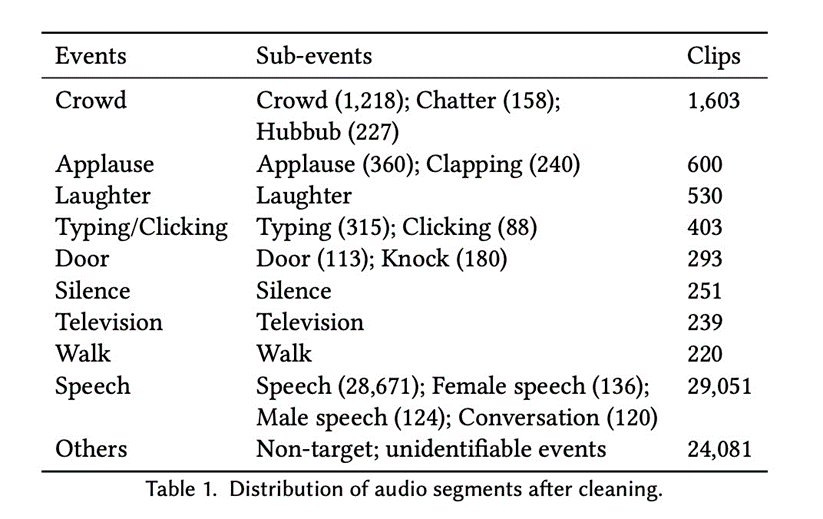
\includegraphics[width=0.7\linewidth]{screenshot001}
	\caption{}
	\label{fig:screenshot001}
\end{figure}

%\section{Context}
%\section{Motivation}
%\section{Hypothesis}
%\section{Client}
%\section{Scope}
\section{Research Questions}

My research questions are:

How can a end-to-end human activity recognition system be built based on ambient audio sensing using mobile devices in a multi-task approach for an office environment?

Sub questions:

\begin{itemize}
	\item What are the current approaches and limitations in the field of activity recognition using acoustic audio?\\
	To answer this question we're going to look at the research.
	\item How can we use multi-task learning to improve acoustic event recognition?\\
	To answer this question we're going to look at the research and find the steps for multi-task learning, as well as check out any approaches that have been tried.
	\item How can a multi-task acoustic event detection system be developed for lifelog modeling in an office environment?\\
	To answer this question we're going to see how we adapt the system to the current dataset and the requirements for a lifelog, as well as try to leverage benefits from knowing it's for an office environment.
	\item How feasible is it to build a multi-task acoustic event classifier for mobile devices? \\
	To answer this question, we're going to build a multi-task classifier as well as a classifier for separate events, check the difference in performance, memory usage and evaluate its feasibility for mobile devices.
\end{itemize}


%\section{Challenges}

%According to \cite{chandrakala2019environmental}, challenges/characteristics in correlation with the scenes:

%\begin{itemize}
%	\item Signal-to-noise ratio (SNR) is typically very small in an audio signal, particularly if the microphone is not very near to the acoustic source (Crocco et al. 2016)
%	\item Discriminative information exists in low-frequency ranges (chachada and Kuo 2014)
%	\item environmental sounds/scenes do not have any specific structures such as phonemes or prosody (Cowling and Sitte 2003).
%\end{itemize}

%Challenges in connection to automatic recognition of audio scenes or events:

%\begin{itemize}
%	\item Recognizing many events from a single environment, such as an office room, a residential area, or a busy street that may have multiple sound sources (Messaros et al. 2010, 2015)
%	\item A dictionary of basic units is unidentifiable (Cowling and Sitte 2003)
%	\item the existence of overlapping or polyphonic events (Gemmeke et al. 2013; Mesaros et al. 2010)
%	\item recognition of confusing scenes e.g. street traffic vs. restaurant (Ntalampiras et al. 2011)
%	\item Lack of discrimination among scenes such as pedestrian street market, quiet street and shop (Rakotomamonjy and Gasso 2015)
%	\item identifying acoustic sound sources in the presence of background noise (Beltran et al. 2015; Salamon et al. 2014)
%	\item The existence of certain audio events in multiple environments, e.g., "gunshot" sound present in environments such as street and home (Heittola et al. 2013)
%	\item The multimodal surveillance systemn for critical indoor environments (Moeslund et al. 2014)
%	\item lack of standard and multimodal datasets (Chchada and Kuo 2013);
%	\item Lack of robust and compact representation learning techniques for audio scenes and sound events. (Ozer et al. 2018; Phan et al. 2017)
%\end{itemize}



\section{Contributions}

My contributions are:

\begin{itemize}
	\item A systematic literature review of the state-of-the-art deep learning approaches in Acoustic Sound Detection (AED) as well as Deep learning multi-Task learning algorithms, as well as investigating the design space for use in lifelogging systems.
	\item A neural network-based multi-task system able to detect and classify multiple overlapping events in audio fragments.
	\item Application and analysis of this classifier on a specific use-case, namely an office environment.
	\item Evaluation of the feasibility to run single and multi-task classifiers on mobile devices. 
\end{itemize}
\section{Outline}




